\documentclass{article}

\usepackage{float}
\usepackage{enumerate}
\usepackage{enumitem}

\IEEEoverridecommandlockouts
% The preceding line is only needed to identify funding in the first footnote. If that is unneeded, please comment it out.
\usepackage{cite}
\usepackage{amsmath,amssymb,amsfonts}
% \usepackage{algorithmic} % Commented out since I didn't have the package and it didn't seem needed
\usepackage{graphicx}
\usepackage{textcomp}
\usepackage{xcolor}

\usepackage{multirow}
\usepackage{rotating}

\usepackage{mdframed}
\usepackage{hyperref}
\usepackage{tikz}
\usepackage{makecell}
\usepackage{tcolorbox}
\usepackage{amsthm}
%\usepackage[english]{babel}
\usepackage{pifont} % checkmarks
%\theoremstyle{definition}
%\newtheorem{definition}{Definition}[section]


\usepackage{listings}

\title{Exercises 2}


 
\author{
    Henrik Schwarz \\ hschw17 
    \and
    Hampus Gärdström \\ hgard20
    \and
    Tom Souček \\ tosou23
    \and
    Henrik Prüß \\ hepru23
    \and
    MD Fahim Shahriar \\ fasha23
    \and
    Tom Bourjala \\ tobou23
}

\begin{document}
\maketitle

\section{Assumptions}
In order to provide context around the system we make assumptions regarding it. We make assumptions regarding the company size and it's production need. Additionally, we also make some assumptions about the production process in regards to technology and requirements.

We assume the the company is a mid-sized company producing bikes and electric bikes for the commercial market. We have made the assumption that it is a mid sized company because the hardware seems expensive and because most smaller companies have no need for a 24/7 production line. Moreover, it does not appear to be a large company as the production line appears small. The assumption that the company produces bikes or electric bikes was made because the tools in the assembly line seems advanced, however this assumption is mostly arbitrary but serves to give an interesting context for the system.

Based on the assumption that the company produces bikes and electric bikes, we further assume that the production line should be able to manipulate parts from metal and plastics to electronics, in a complex assembly and treatment process. In the process of this we assume that there is a need for many different technologies along the assembly line, which we assume would create a strong need for middleware.
We also assume that the production line should concern itself with being able to recover unfinished products that may come from an emergency stop or an unexpected breakdown. In such cases, we assume that it would be reasonable for it to automatically recover or discard the products when resuming operations.
Furthermore, it would be important to allow for the addition or variation of modules in the assembly line. This would be important in order to accommodate changing production needs.
We assume that  system needs to concern itself with security and safety of human actors during production due to compliance. This could cause a need for emergency stops or automatic proximity shutdowns.

\section{Use Cases}
\begin{table}[H]
\caption{Extensibility and flexibility use case}
\centering
\begin{tabular}{|l|p{8cm}|} \hline
Name & Introduction of a new bike model \\ \hline
Actors & Assembly technician, production manager, production scheduler \\ \hline
Pre condition & A design of the new bike, specifying the required production  \\ \hline
Description & \begin{enumerate} 
\item The production manager logs into the the production software.
\item The production manager configures a new production step in the software.
\item The production manager asks the assembly technician to add new hardware to the assembly line.
\item The assembly technician installs hardware to the assembly line.
\item The production manager configures a new production run including the new production step in the software.
\item The production manager schedules a test run.
\item The production scheduler confirms the test schedule and starts the production run.
\item The assembly technician and production manager confirm the correctness of the newly established production run.
\end{enumerate} \\ \hline
Post condition & A new bike resembling a test artifact of the newly established production run. \\
\hline
\end{tabular}
\end{table}

\begin{table}[H]
\centering
\caption{Security use case}
\begin{tabular}{|l|p{8cm}|} \hline
Name & Emergency shutdown due to malfunctioning test bench \\ \hline
Actors & Test bench, quality assurance worker \\ \hline
Pre condition & QA Worker performs quality assurance of the produced bike at a test bench. The test bench includes the use of robotic arms for easier inspection of the bike.  \\ \hline
Description & \begin{enumerate} 
 \item The quality assurance worker starts his inspection of the produced bike. Therefore, he uses a test bench that utilizes robotic arms enabling easier inspection of the bike (i.e. the robotic arms help to lift, rotate, etc. the bike).
\item While standing very close to the bike, the robotic arms begin to move the bike in unpredictable ways.
\item Sensors detect the proximity of the human worker to the malfunctioning machine.
\item The security system interprets it as threat to the human worker.
\item The security system shuts the malfunctioning test bench down and reports the shutdown to the supervisory system.
\end{enumerate} \\ \hline
Post condition & The production machine is shutdown and remaining work is load-balanced to the other machines that are available. \\
\hline
\end{tabular}
\end{table}

\begin{table}[h]
\caption{Availability use case}
\centering
\begin{tabular}{|l|p{8cm}|} \hline
Name & Failure of one of the robotic arms. \\ \hline
Actors & Robotic arm, Monitoring system \\ \hline
Pre condition & Production line is running  \\ \hline
Description & \begin{enumerate} 
    \item The robotic arm is doing a rutine task it has been programmed for.
    \item The robotic arm suddenly encounters an error that causes it to malfunction.
    \item The robotic arm goes into safe mode and notifies the monitoring system.
    \item The Monitoring system notices that the robot is malfunctioning and creates a ticket for the a need of repair for the arm(Which system?).
    \item The Monitoring system tries to find another robot that can do the job of the arm.
    \item The Monitoring system finds another arm that can take the job of the malfunctioning arm.
    \item The other robotic arm picks up the load from the malfunctioning arm.
\end{enumerate} \\ \hline
Post condition & The system keeps runnng with the other arm is doing the job of the malfunctioning and there is a ticket about the malfunctioning robot in the system. \\
\hline
\end{tabular}
\end{table}

\begin{table}[h]
\caption{Recoverability use case}
\centering
\begin{tabular}{|l|p{8cm}|} \hline
Name & Power outage interrupts the production line \\ \hline
Actors & Production line \\ \hline
Pre condition & The production line is running.  \\ \hline
Description & \begin{enumerate} 
\item The area for the production line encounters a loss of power for 5 minutes.
\item The power is back on again.
\item The production line is starting up again.
\item The production line queries the supervisor system for what the current task is and what the last state was.
\item The supervisor system responds with the details.
\item The product line uses the details from the supervisor system to resume activity
\end{enumerate} \\ \hline
Post condition & The product line is running again and continuing as normal. \\
\hline
\end{tabular}
\end{table}


\begin{table}[h]
\caption{Use case for a customer checking on the progress of their bike.}
\centering
\begin{tabular}{|l|p{8cm}|} \hline
Name & Checking the progress on a bike order\\ \hline
Actors & Customer, webshop(?), Order system \\ \hline
Pre condition & The order for the bike has been processed.  \\ \hline
Description & \begin{enumerate} 
    \item The Customer wants to check the progress of their bike order.
    \item The customer logs into the webshop interface.
    \item The customer goes to their order page.
    \item The customer clicks on their order.
    \item The webshop quries the Order system to get the status of the order.
    \item The Order system responds with the status of the order. 
    \item The webshop uses the order status to show the order
    \item The customer can see the progress of the order.
    \item The customer logs out of the system.
\end{enumerate} \\ \hline
Post condition & The customer has the information on the progress of their bike. \\
\hline
\end{tabular}
\end{table}

\section{Systems and subsystems}
For our bike manufacturing company, we have defined 3 primary systems that will be discussed in this section. These systems should be sufficient to accept an order, manage the supply of all materials, and manage the whole production line.

\subsection{Enterprise resource system}
First to mention is an enterprise resource system whose first step is to receive orders. After an order is received the system generates an invoice for the customer and tries to predict the time needed to complete the bike. This estimate is based on other subsystems such as the production capacity system or human resource planning system. In case of unhappy customers, this system also handles customer support including accepting the complaint and assigning it to employees.

\subsection{Suply chain management system}
This system is used to manage the supply chain and logistics. Part of the logistics is ensuring that there is enough material in the warehouses -- this is managed by an inventory subsystem. If there are materials missing and need to be ordered that's when the procurement subsystem comes in handy. This subsystem consists of a blockchain of vendors and a tracking system which helps us with planning. Since we consider collecting data from various suppliers there is also a quality history system helping with decision-making when it comes to choosing a supplier.

\subsection{Production management system}
This is the system where the actual production of a bike takes place. Apart from the production itself, also a scheduling system is a must, in order to achieve maximal efficiency. Another mentionable subsystem is quality control where it is ensured that every bike meets industry standards. It is inevitable that there might occur some errors in the production line and therefore there is also an existence of an error handling system ensuring fault correction and recovery. Integration of some bike components can´t be assembled fully by robots and that is when assembly technicians come in. That creates a need for safety requirements ensuring no human is harmed. That is a responsibility of a security system.
\begin{figure}[H]
    \caption{Diagram of our system for a bike assembly line.}
    \centering
    \begin{sideways}
        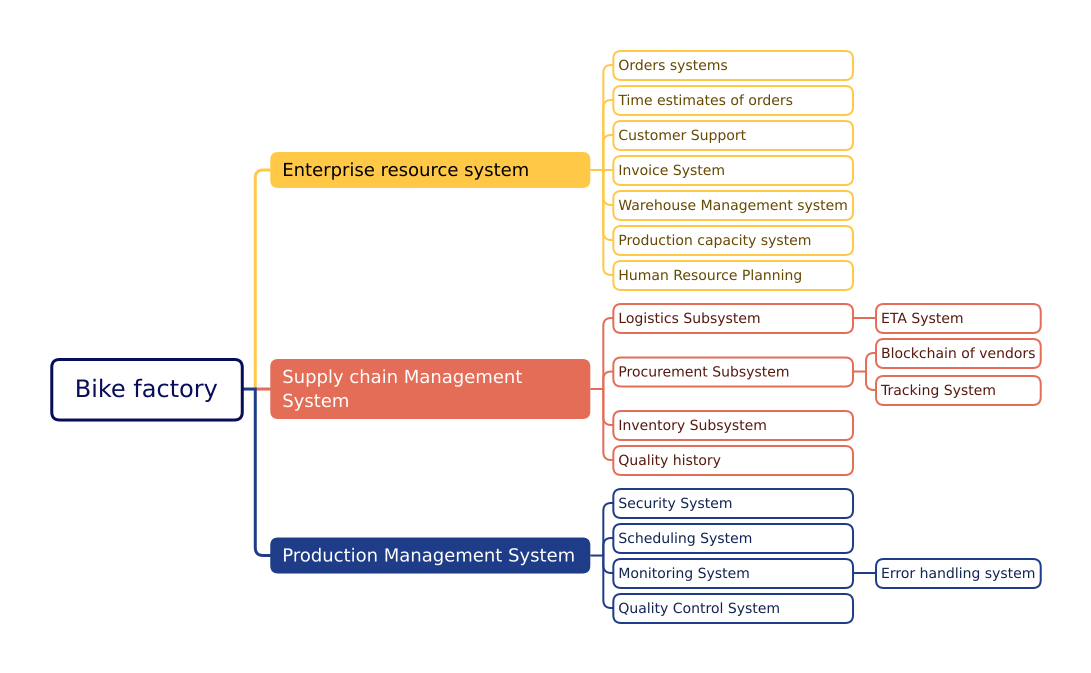
\includegraphics[scale=0.5]{diagram.png}    
    \end{sideways}
    \label{fig:enter-label}
\end{figure}



\end{document}

